\section{检修方案设计(问题三)} % (fold)
\label{sec:检修方案设计}

为了保障生产安全、提高工厂生产条件,生产工厂常常有计划地对关键设备进行检修升级。
对关键设备的检修势必会影响其正常生产,因此有必要针对工厂具体生产条件,合理设计检修安排,保证工厂安全、高效运转。

\subsection{模型的建立与求解} % (fold)
\label{sub:模型的建立与求解}

题目要求制定生产工厂停工检修计划,并使总成本最小。
为了表示当天$t$是否检修,本文引入了0$\textendash$1变量$\mu_t$,等于1表示当天进行检修,等于0表示不进行检修

\begin{equation}
	\mu_{t} \in\{0,1\},\quad t=1,2,\cdots,210.
\end{equation}

总共设置7次停工检修,每次检修时间为1天,故有:

\begin{equation}
	\sum_{t=1}^{210}\mu_t=7.
\end{equation}

生产工厂在检修日无法生产,且两次检修需彼此间隔6天及以上。
\begin{equation}
	\sum_{t=i-5}^{i} \mu_{t} \leqslant 1,\quad i=6,7, \cdots, 210.
\end{equation}
上式中,通过对任意6天内检修与否逻辑变量$\mu_t$进行求和,以检验检修日间隔长度,保证检修日间隔符合题目要求。

检修之后,工厂关键设备生产效率会略有上升(工时限制放宽10\%),并以2\%/天的速率衰减到0。
因此,需对问题一中式\ref{修正式}总工时限制:
\begin{equation}
	\sum_{r=1}^{R} M_{t}^{r} \leqslant M_{t}.
\end{equation}
进行修正,得:
\begin{equation}
	\sum_{r=1}^{R} M_{t}^{r} \leqslant M_{t}\left(1-\mu_{t}+0.1 \mu_{t-1}+0.08 \mu_{t-2}+0.06 \mu_{t-3}+0.04 \mu_{t-4}+0.0 \mu_{t-5}\right).
\end{equation}
其中,$M_{t}^{r}$表示第$t$天、组件$r$的生产工时花费,
$M_{t}$表示计划中第$t$天生产总工时限制。

另外,本题不将一周视为一个生产周期,而将30周(共210天)视为整体,故$T=210$.

综上,得到线性模型如下:

\begin{equation}\label{三模型}
	\begin{aligned}
&\min \quad z  = \sum_{t  = 1}^{T} \sum_{r = 1}^{R}\left(s^{r} \omega_{t}^{r}+h^{r} y_{t}^{r}\right)\\
& \ \begin{array}{r@{\quad}l@{}l@{\quad}l}
\mathrm{s.t. }
&	\sum_{r=1}^{R} M_{t}^{r} \leqslant M_{t}(1-\mu_{t}+0.1 \mu_{t-1}+&0.08 \mu_{t-2}+0.06 \mu_{t-3}+0.04 \mu_{t-4}+0.0 \mu_{t-5});\\
&M_{t}^{r} \leqslant M_{t}^{r} \omega_{t}^{r}, &t=1,2, \cdots, T, r=1,2, \cdots, R;\\
& y_{t}^{r}=y_{t-1}^{r}+x_{t}^{r}-\eta_{r}^{r} x_{t}^{r^{\prime}}, &t=1,2, \cdots, T,  r=1,2, \cdots, R; \\
&\mu_{t} \in\{0,1\};&\\
&\sum_{t=1}^{210}\mu_t=7;&\\
&\sum_{t=i-5}^{i} \mu_{t} \leqslant 1,& i=6,7, \cdots, 210;\\

&\omega_{t}^{r} \in\{0,1\}, &t=1,2, \cdots, T, r=1,2, \cdots, R; \\
&x_{t}^{r}=x_{t}^{r} \omega_{t}^{r},&t=1,2, \cdots, T, r=1,2, \cdots, R;\\
&c^{r} x_{t}^{r}=M_{t}^{r} \omega_{t}^{r}, &t=1,2, \cdots, T, r=1,2, \cdots, R; \\
&M_{t}^{r} \geqslant 0,& r=1,2, \cdots, R ;\\
% &y_{0}^{r}=y_{T}^{r}=0,& r=1,2, \cdots, R ;\\
&x_{t}^{r}, y_{t}^{r} \geqslant 0, &t=1,2, \cdots, T, r=1,2, \cdots, R;\\
&y_{t-1}^{\mathrm{WPCR}}+x_{t}^{\mathrm{WPCR}}-y_{t}^{\mathrm{WPCR}}=d_{t}, & t=1,2, \cdots, T; \\
&\eta_{r^{\prime}}^{r} x_{t}^{r^{\prime}} \leqslant y_{t-1}^{r}, &t=1,2, \cdots, T, r=1,2, \cdots, R;
\end{array}.
\end{aligned}
\end{equation}

\subsection{检修方案展示} % (fold)
\label{sub:检修方案展示}


\begin{figure}[!htbp]
	\centering
	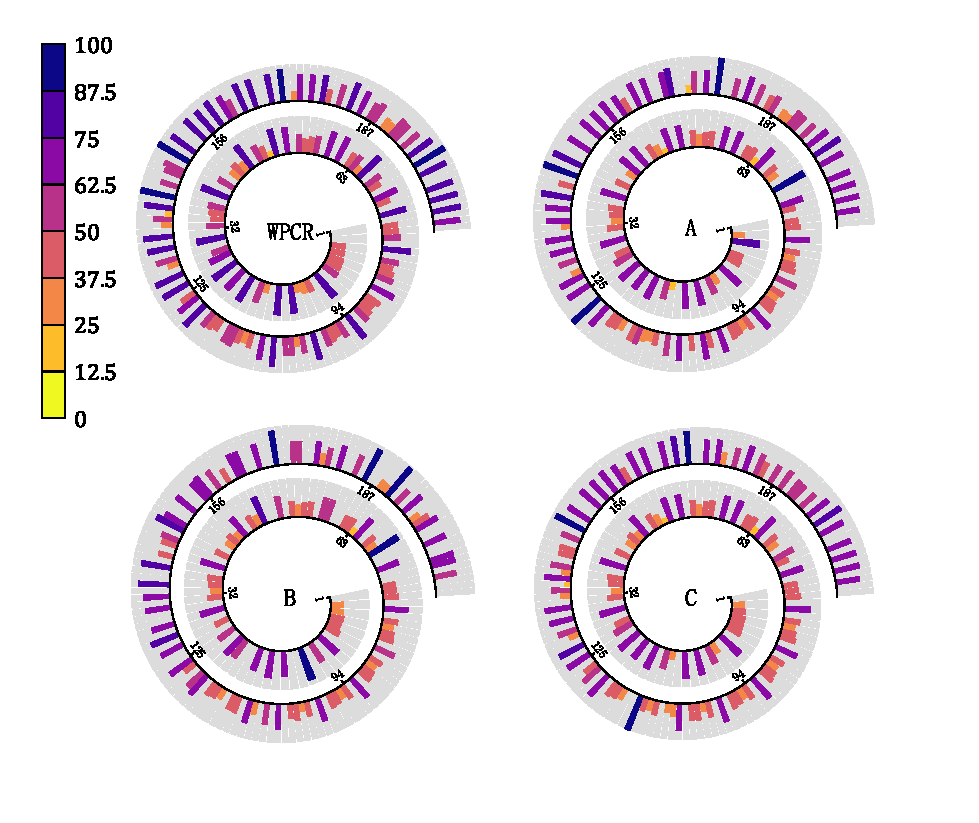
\includegraphics[width=16cm]{Image/问题三展示.eps}
	\caption{问题三}\label{问题三}
\end{figure}

\begin{table}[!htbp]
\centering
\caption{检修日期及总成本}
\resizebox{\linewidth}{!}{
\begin{tabular}{cccccccl}
\toprule[1.5pt]
\multicolumn{7}{c}{检修日安排}                             & \multicolumn{1}{c}{总成本}      \\
\midrule[1pt]
第 1 次 & 第 2 次 & 第 3 次 & 第 4 次 & 第 5 次 & 第 6 次 & 第 7 次 & \multirow{2}{*}{$5.3\times10^6$}  \\
\cline{1-7}
1     & 37    & 44    & 51    & 65    & 86    & 210   &                              \\
\bottomrule[1.5pt]
\end{tabular}
}
\end{table}

事实上,由于本文并未求得问题3的全局最优解,因此分析得到的局部最优解的意义是有限的.
因为边界条件约束了周一不能进行生产工作,所以将第一次检修安排在周一几乎是必然的.
根据前两问的经验,最后一天一般也不进行生产工作,故安排最后一次检修也不会损失产量,但也浪费了检修带来的产能提升.
由表四可知,其余检修安排在了生产中前段,且十分密集,猜测与求解器的逻辑有关.
以上安排的内在深层次原因,笔者希望在之后求得最优解后继续研究,以期得到满意解释.

% subsection 检修方案展示 (end)
% subsection 模型的建立与求解 (end)
% section 检修方案设计 (end)
